% TEMPLATE for Usenix papers, specifically to meet requirements of
%  USENIX '05
% originally a template for producing IEEE-format articles using LaTeX.
%   written by Matthew Ward, CS Department, Worcester Polytechnic Institute.
% adapted by David Beazley for his excellent SWIG paper in Proceedings,
%   Tcl 96
% turned into a smartass generic template by De Clarke, with thanks to
%   both the above pioneers
% use at your own risk.  Complaints to /dev/null.
% make it two column with no page numbering, default is 10 point

% Munged by Fred Douglis <douglis@research.att.com> 10/97 to separate
% the .sty file from the LaTeX source template, so that people can
% more easily include the .sty file into an existing document.  Also
% changed to more closely follow the style guidelines as represented
% by the Word sample file. 

% Note that since 2010, USENIX does not require endnotes. If you want
% foot of page notes, don't include the endnotes package in the 
% usepackage command, below.

% This version uses the latex2e styles, not the very ancient 2.09 stuff.
\documentclass[letterpaper,twocolumn,10pt]{article}
\usepackage{usenix,epsfig,endnotes}
\begin{document}

%don't want date printed
\date{}

%make title bold and 14 pt font (Latex default is non-bold, 16 pt)
\title{\Large \bf The Effect of Virtualization in Timing Filesystem Operations}

%for single author (just remove % characters)
\author{
{\rm Rob Jellinek}\\
\and
{\rm Adam Vail}\\
% copy the following lines to add more authors
% \and
% {\rm Name}\\
%Name Institution
} % end author

\maketitle

% Use the following at camera-ready time to suppress page numbers.
% Comment it out when you first submit the paper for review.
\thispagestyle{empty}


\subsection*{Abstract}

\section{Introduction}

In recent years large and small businesses have demanded cost effective ways of increasing their computing power.
This has led to the proliferation of full hardware virtualization.
Virtualizing computing resources has revolutionized the current environment in two distinct ways.
It has allowed companies to fully utilize their current systems by combining many machines onto a single physical system.
It has also produced new business models where companies flexibly rent computing time to customers who can pay for only what they need.

\paragraph{}
In order to run unaltered commodity operating systems, the virtual machine monitor must fully virtualize the system's underlying hardware.
This leads to the question of what happens when software that assumes it is running directly on bare hardware is run in a virtualized environment?
Therefore, we studied the effects of virtualization on the ext2 file system.
We studied four specific characteristics of ext2, comparing its performance when running on bare metal and when running in a virtual machine.

\paragraph {}
The first characteristic that was measured was the ideal buffer size when randomly reading from a file. 
Random reads can be very costly since in the common case, the desired data will not be in the cache. 
Knowing the amount of data that can be retrieved for the lowest cost allows the user to extract the highest performance out of the file system when creating applications with large amounts of random reads. 
The experiment tested different buffer lengths at different increments. 
It was determined that for both bare metal and virtual, buffers under 4096 bytes in size perform similarly when randomly reading from a file. 
Buffers over 4096 bytes in size require an increase in cycles to read all the data. 
This buffer size represents the block size for the file system. 
When ext2 reads and writes to disk it does so at the block level.
Blocks are a foundational element in file system and this value is significant because it is then used in all other file system measurements.

\paragraph{}
The second characteristic measured was the amount of data prefetched by the file system. 
When reading from a disk, the file system assumes the user will most likely read data sequentially. 
In order to increase performance for this common case the file system reads extra blocks that are located after the requested data. 
This is useful because it allows the user to read sequentially without constantly paying the penalty for having to go out to disk. 
Again, the experiment yielded results indicating that ext2 behaves similarily in both environments, prefetching 128 KB of data whenever a block is read from disk.

\paragraph{}
The third characteristic measured was the size of the file system cache. 
This is particularly important to the user since it indicates the amount of data that they can access without incurring large delays. 
It is not a uniform characteristic across all instances of ext2 since the size is related to the amount of free memory in the system. 
%% TODO New values for thisi, compare virt and bare --  The experiment was run on a system containing 4 GB of memory resulting in a cache size of about 3.3 GB.

\paragraph{}
The final characteristic measured was the file size at which ext2 requires indirection to store data. 
Since ext2 uses inodes to organize data on disk, the number of pointers in the inode that directly reference data determines the largest file size before needing to use indirection. 
Then, extra layers of indirection are used as the file size increases. 
Ext2 implements three levels of indirection which allows for file sizes up to 2 TB (depending on the block size). 
The experiment showed that ext2 uses twelve direct inodes. 
Therefore, an inodes can directly reference a file of up to 48 KB. 
%% TODO compare virt and bare

\section{Methodology}
\subsection{Environment}
All experiments, both on bare metal and virtual, were run using 64-bit Ubuntu 12.04 (Linux 3.2.0-30-generic kernel) and the ext2 file system.
The system used an Intel Core i5 2.8 GHz quad-core processor with Intel VT enabled and 6 GB of memory.
Virtualization was done via KVM (Kernel-based Virtual Machine) which offers full virtualization of the x86 hardware.
The virtual machine was configured with 6 GB of memory and a single processor.
Additional memory was installed in the test machine to allow the virtual machine to have an equal amount of memory as the bare metal machine.
Experiments on the virtual machine were run with an underlying test system that was equipped with 12 GB of memory.
All experiments were implemented in C and identical between the bare and virtual environments. 
The experiements were run with the taskset and nice commands in order to affinitize the experiment to a single CPU and set its priority as high as possible.
The cache was dropped between runs of every experiment using the \texttt{drop\_caches} ability provided by the kernel.
The ext2 file system was on a SATA connected 500 GB Western Digital Caviar Green drive. 
The Caviar Green family of disks adjusts the speed of the drive in order to save power. 
This power saving mode goes into effect after eight seconds of inactivity.
The first run of every experiement was used to "wake up" the drive and was subsequently thrown out due to needing "spin-up" time. 

\paragraph{}
The timer used for all experiments was the time stamp counter which was accessed through the rdtsc instruction provided by the Intel instruction set. 
This is called in C by designating the command as assembly. 
The command allows access to the cycle count which was used to determine how many cycles it took for an operation to complete. 
This does have the potential to introduce some noise since the CPU is not restricted to run at a fixed frequency. 
Discarding the first run of every experiment helps minimize this inconsistency. 
The timer was tested against the gettimeofday() command. 
The test program slept for several seconds and both the time stamp counter and gettimeofday determined the same amount of sleep time. 
Although, each core in a multi core processor has its own time stamp counter.
Therefore, each experiment had to be affinitized to a single core to ensure the accuracy of the timing. 

\subsection{Measuring the Ideal Buffer Size for Random Reads}

In order to determine the ideal buffer size when performing random reads, reads of various sizes were performed and the times for each read were compared. 
Since this measurement is essentially determining the block size, if bytes are read from the same block then they should have fast access times. 
Once the file system needs to read from a new block it will have to fetch that block before returning the data. 
Therefore, when the read time increases significantly it is the start of a new block.
Reads were started from a block chosen randomly within the first 1000 blocks of the file and were done in reverse order to counteract prefetching. 
Since the default page size for the Linux kernel is 4 KB, it is logical that the file system make this its basic unit for moving data. 
Therefore we expected the ext2 block size to be 4096 bytes.

\subsection{Measuring the Amount of Data Prefetched by the File System}
When a block is read from the disk the file system makes the assumption that the data following that block is going to be read in the near future. 
Thus, when a block is read, some number of subsequent blocks are cached so that when the application reads these blocks they can be returned much faster than going out to disk. 
The experiment randomly chose a block to read from the first one thousand blocks of the file. 
It then slept for one second in order to allow for all the prefetched data to be put into the cache. 
It then sequentially read the blocks following the initial block and timed how long it took for that block to be read. 
Blocks in the cache should be returned very quickly. 
A long read time for a block indicates that the file system had to go out to disk in order to retrieve it. 
Along with retrieval of that block the file system would again prefetch data. 
Therefore the expected timing distribution was a consistent number of fast reads (blocks in the cache) separated by spikes indicating the file system had to go out to the disk. 
The number of blocks from one spike to the next revealed the size of the prefetch.

\subsection{Measuring the Cache Size}
The cache allows the file system to keep recently accessed (and potentially soon to be accessed due to prefetching) data in memory. 
By not having to go out to disk on a request it speeds up the retrieval time immensely. 
The size of the cache is affected by the amount of free physical memory in the system. 
The system we used for our experiments typically had two 6GB DIMMs. In order to speed up test times and to provide a similar environment for the native and virtual settings, we removed a DIMM for our native tests, so that the native machine was running on a total of 6GB of physical memory. In our VM-based tests, we inserted both DIMMs so that the machine had 12GB of physical memory, but only made 6GB available to the virtual machine. Otherwise, with only one DIMM installed for the VM tests, we would have been unable to allocate the full 6GB to the guest VM.
%Both the bare metal system as well as the virtual machine had 6 GB of memory and no extra applications running. 
We also consider that there is a source of noise in that operating system processes were running at the time of the experiments, thus taking up some amount of memory.
The experiments were run in a consistent environment in order to try and control the noise as much as possible. 
With 6 GB of memory it was expected that the cache would take up the majority of the free space and have a size near 5 GB. 
This was tested by doing repeated reads to the same blocks of data. 
Blocks in the cache have very fast read times. 
Once the amount of data being read is too large to fit inside the cache, the read times increase as the file system has to continually go out to disk due to cache misses. 
Prefetching was controlled by reading all the desired blocks initially without timing to allow for the data to be placed in the cache. 
Then, the same data was read again while being timed. 
All individual reads were of block size in order to avoid allocating large amounts of space on the heap and unnecessarily consuming memory.

\subsection{Inode Indirection}
%% TODO once we figure out what is going on here


\section{Results}

\subsection{Buffer Size}
\begin{figure}[!ht]
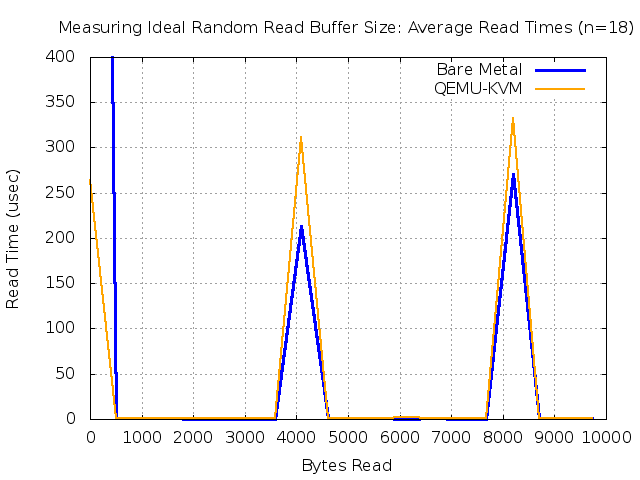
\includegraphics[scale=.35]{random_avg.png}
\caption{Ideal buffer size for random file access: average read times}
\end{figure}
\begin{figure}[!ht]
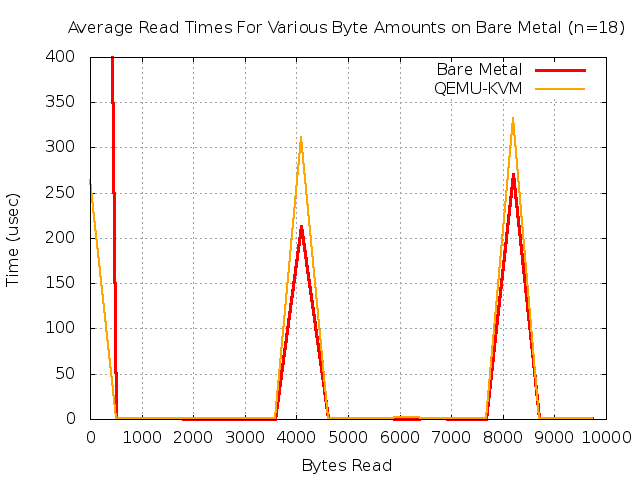
\includegraphics[scale=.35]{random_combined.png}
\caption{Ideal buffer size for random file access: combined read times}
\end{figure}

When reading 512-byte blocks in reverse starting from a random point in our target file on ext2, read times jumped on 4096-byte boundaries. On bare metal, average read times jumped from approximately 0.5 microseconds when the read happened within a 4k block, to 200-250 microseconds for the first read into a new 4k block. Under QEMU-KVM, read times within a block  took approximately 0.75 microseconds and jumped to 300-400 microseconds for the first read into a new 4k block.  

This is consistent with our hypothesis that read times would spike on the first read into a new block but remain low otherwise. Since ext2 defines a block size as 4096 bytes, the first read into a new block fetches the block from disk into memory; all subsequent reads from that block can be done directly from memory, and so are much quicker.

The consistency is spikes, but relative difference in latency between our bare-metal and QEMU-KVM tests are also consistent with our expectations. Virtio implements virtual queues that serve as an interface between a set of front-end drivers in QEMU, and back-end drivers in the KVM hypervisor. I/O requests and responses are passed between guest and host first via the virtio-blk device driver and then through these queues to the hypervisor, where the actual I/O request is then made and the result is returned to the guest. The additional time required to transfer the I/O request and response would explain the higher response time observed under QEMU-KVM when compared with bare metal. In particular, the greater relative slowdown when a block is newly fetched from disk (~100 microsecond difference between bare metal and VM), compared with when data is fetched from memory (~0.25 microsecond slowdown for the VM) is in line with expectations. 

\subsection{Prefetching}
\begin{figure}[!ht]
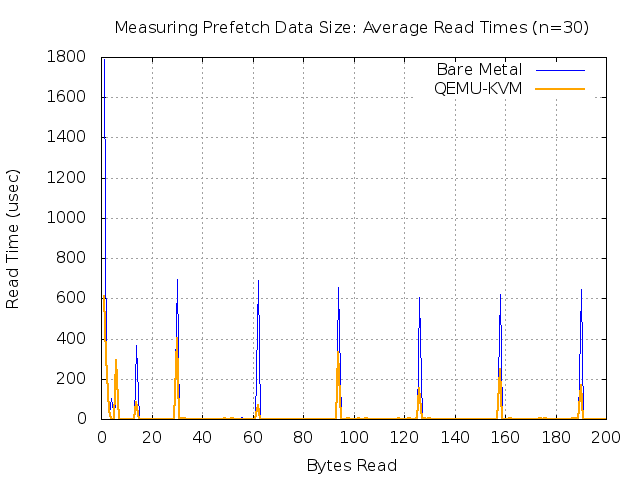
\includegraphics[scale=.35]{prefetch_avg.png}
\caption{Measuring sequential reads to determine prefetching size: average read times}
\end{figure}
\begin{figure}[!ht]
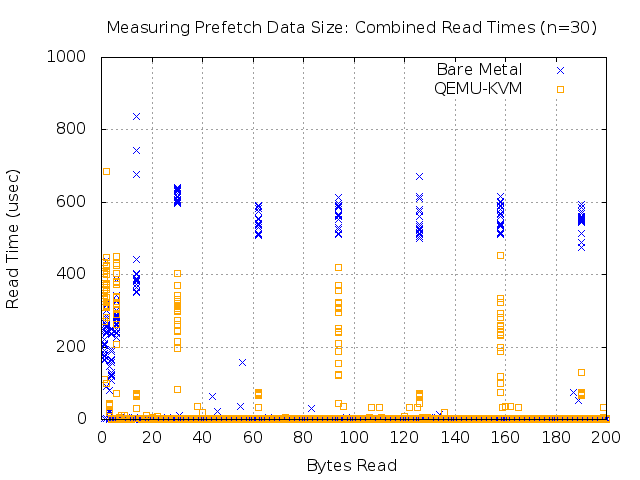
\includegraphics[scale=.35]{prefetch_combined.png}
\caption{Measuring sequential reads to determine prefetching size: combined read times}
\end{figure}
Our results confirmed our hypothesis that read times would be fast for some set number of blocks corresponding to the number of blocks prefetched ahead on a sequential read, and would spike when the next set of blocks had to be read from disk. Our results show the high read times occur at 32-block intervals, indicating that ext2 prefetches 128k of data at a time. We found that read times rose to from approximately 1 microsecond to 500-600 microseconds on bare metal, and from approximately 1 microsecond to 150-400 microseconds on QEMU-KVM. 

While the amount of data prefetched was consistent between the native and virtualized settings, the relative difference in the time it took to read from disk is very surprising. It is unclear why reading data from disk in the virtual setting would occur \textit{with lower latency} than when performing the same read in the native setting. 
%% TODO: finish/clarify the above.

\subsection{File Cache}
\begin{figure}[!ht]
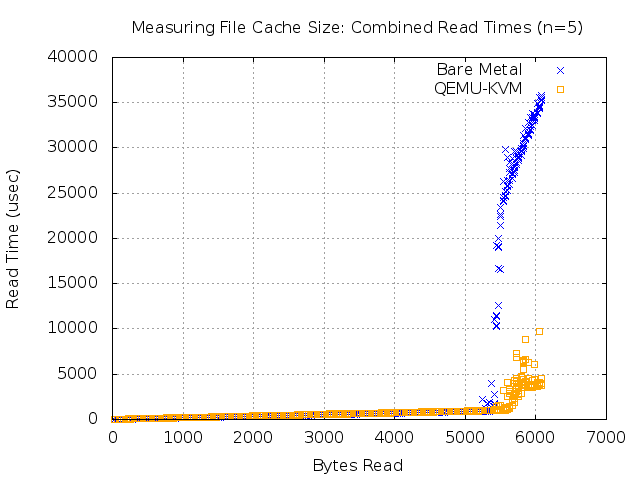
\includegraphics[scale=.35]{cache_combined.png}
\caption{Measuring file cache size: combined read times}
\end{figure}
Figure 5 shows the results from our cache-timing tests in the native and virtual settings. Both settings show very low read times for the first 5.3GB of data, implying that it fit in the file cache. We can assume that the remaining physical memory was consumed by background processes and kernel data structures. After the first 5.3GB, the read time for additional bytes skyrockets in the native setting, but remains relatively low in the virtual setting. This is most likely attributable to our experimental setup, where we had only one 6GB DIMM in the native setting, but two 6GB DIMMs in the virtual setting (though we only allocated the 6GB to the VM). 

%TODO: Is the following correct or plausible? Potentially talking out my a**. Especially toward the end.
In the native setting with 6GB of physical memory, assuming the file cache was 5.3GB and background processes and the kernel filled the remaining space, no additional files could be cached in physical memory past the 5.3GB mark. Reading additional files would require going to disk in each case, swapping out old data from the cache, and replacing it with the new data read, all of which is very expensive. In the VM setting, however, since we actually have 12GB of physical RAM, the VM will fill up its own file cache, which appears to be slightly larger than that from the native setting (probably because the bare linux installation in the VM had fewer modules/background processes loaded). But then when it tries to read an additional file, it is cached in the remaining free physical memory of the hypervisor--outside the 6GB visible to the guest VM, but accessible now only with the overhead required to swap the page in from the hypervisor's memory into the guest OS's memory. If read pages are shared, this may not even involve a swap, but only a page-table update. 

\subsection{Inode Indirection}

\section{Conclusions}

{\footnotesize \bibliographystyle{acm}
\bibliography{../common/bibliography}}

\theendnotes

\end{document}







